\setlength{\parindent}{0cm}
\setlength{\parskip}{1ex plus 0.5ex minus 0.2ex}
\newcommand{\hsp}{\hspace{20pt}}
\newcommand{\HRule}{\rule{\linewidth}{0.5mm}}
\begin{titlepage}
  \begin{sffamily}
  \begin{center}

    
\includegraphics[scale=0.2]{logo.jpg}~\\[2cm]

    \textsc{\LARGE Université de Nantes}\\
    \textsc{\LARGE  }\\
    \textsc{\Large UFR Sciences et Techniques}\\
    \textsc{\LARGE  }\\
    \textsc{\LARGE  }\\
    \textsc{\Large Algorithmique et programmation avancées pour les biologistes}\\
    \textsc{\LARGE  }\\
    \textsc{\Large Algorithmes et méthodes pour la Bio-Informatique}\\[1cm]

    % Title
    \HRule \\[0.4cm]
    { \huge \bfseries Extraction de motifs communs à plusieurs séquences biologiques\\[0.4cm]
     }
    \HRule \\[2cm]

    % Author and supervisor
     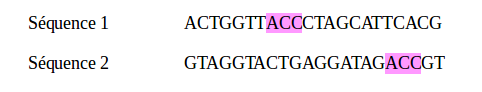
\includegraphics[scale=0.7]{deco.png}~\\[2cm]
    
 
      \begin{center} \large
       Ulysse \textsc{Guyet}\\
       Jennifer \textsc{Rondineau}\\
       Master 2 Bioinformatique \\
      \end{center}

    \vfill

    % Bottom of the page
    {\large 16 décembre 2015}

  \end{center}
  \end{sffamily}
\end{titlepage}
